\documentclass{article}\usepackage[]{graphicx}\usepackage[]{color}
% maxwidth is the original width if it is less than linewidth
% otherwise use linewidth (to make sure the graphics do not exceed the margin)
\makeatletter
\def\maxwidth{ %
  \ifdim\Gin@nat@width>\linewidth
    \linewidth
  \else
    \Gin@nat@width
  \fi
}
\makeatother

\definecolor{fgcolor}{rgb}{0.345, 0.345, 0.345}
\newcommand{\hlnum}[1]{\textcolor[rgb]{0.686,0.059,0.569}{#1}}%
\newcommand{\hlstr}[1]{\textcolor[rgb]{0.192,0.494,0.8}{#1}}%
\newcommand{\hlcom}[1]{\textcolor[rgb]{0.678,0.584,0.686}{\textit{#1}}}%
\newcommand{\hlopt}[1]{\textcolor[rgb]{0,0,0}{#1}}%
\newcommand{\hlstd}[1]{\textcolor[rgb]{0.345,0.345,0.345}{#1}}%
\newcommand{\hlkwa}[1]{\textcolor[rgb]{0.161,0.373,0.58}{\textbf{#1}}}%
\newcommand{\hlkwb}[1]{\textcolor[rgb]{0.69,0.353,0.396}{#1}}%
\newcommand{\hlkwc}[1]{\textcolor[rgb]{0.333,0.667,0.333}{#1}}%
\newcommand{\hlkwd}[1]{\textcolor[rgb]{0.737,0.353,0.396}{\textbf{#1}}}%
\let\hlipl\hlkwb

\usepackage{framed}
\makeatletter
\newenvironment{kframe}{%
 \def\at@end@of@kframe{}%
 \ifinner\ifhmode%
  \def\at@end@of@kframe{\end{minipage}}%
  \begin{minipage}{\columnwidth}%
 \fi\fi%
 \def\FrameCommand##1{\hskip\@totalleftmargin \hskip-\fboxsep
 \colorbox{shadecolor}{##1}\hskip-\fboxsep
     % There is no \\@totalrightmargin, so:
     \hskip-\linewidth \hskip-\@totalleftmargin \hskip\columnwidth}%
 \MakeFramed {\advance\hsize-\width
   \@totalleftmargin\z@ \linewidth\hsize
   \@setminipage}}%
 {\par\unskip\endMakeFramed%
 \at@end@of@kframe}
\makeatother

\definecolor{shadecolor}{rgb}{.97, .97, .97}
\definecolor{messagecolor}{rgb}{0, 0, 0}
\definecolor{warningcolor}{rgb}{1, 0, 1}
\definecolor{errorcolor}{rgb}{1, 0, 0}
\newenvironment{knitrout}{}{} % an empty environment to be redefined in TeX

\usepackage{alltt}

\usepackage{float}
\usepackage{hyperref}

% Set the margins on the page to not be so large
\addtolength{\oddsidemargin}{-.875in}
\addtolength{\evensidemargin}{-.875in}
\addtolength{\textwidth}{1.75in}
\addtolength{\topmargin}{-.875in}
\addtolength{\textheight}{1.75in}

\hypersetup{
    colorlinks=true,
    linkcolor=blue,
    filecolor=magenta,
    urlcolor=blue,
    citecolor=blue
}

% Take off page numbering
\pagenumbering{gobble}
\IfFileExists{upquote.sty}{\usepackage{upquote}}{}
\begin{document}

\title{%
  Stat 5100 in R: Setup and Introduction \\
}
\date{}

\maketitle

\tableofcontents

\section{Introduction}

As of Spring 2021, the Stat 5100 course is being offered in R for the very first time. You have the option to complete this course in either SAS or R. Both languages are very popular and useful for the material you will learn in this class, but are very different in style.

Here are the main things you should know about each language:

\bigskip

\textbf{SAS}
\begin{itemize}
  \item Costs a lot of money (You get to use SAS for free in this class because you are affiliated with an academic institution)
  \item Very useful ``out of the box.'' Many powerful features are available right away.
  \item Commonly used at large corporations with large datasets.
  \item The syntax (the rules of the language) are incredibly different from nearly every other programming language, so learning SAS will not necessarily help you learn general programming skills.
  \item The philosophy of SAS is ``let's give you a huge amount of output, we'll let you figure out which parts of the output you need.'' If you create a regression model in SAS, you will be thrown a huge amount of output and diagnostics right away by default. Although the large amount of output can feel overwhelming, it can be very nice to have when you're not sure what you're looking for.
\end{itemize}

\medskip

\textbf{R}
\begin{itemize}
  \item Completely free and open-source for everyone.
  \item A very lightweight and small language (compared to SAS), so many powerful features are not available natively.
  \item The most commonly used language for data science and statistics in both academia and industry. Behind Python, R is the second most commonly used language for data science in industry. (We would love to offer this course in Python eventually!)
  \item The syntax of R is similar to some other scripting languages such as Python, so learning R will help you learn general programming skills.
  \item Requires stronger programming skills to get started.
  \item The philosophy of R is ``We assume you know what you're looking for, so we're going to give you the bare minimum.'' In contrast with SAS, R does not give very much output and diagnostics. To obtain the same things that SAS gives you, you must know exactly what you are looking for and run appropriate functions to give you the output you want.
  \item To expand the power of R, we use what are called ``packages.'' Packages are code that is written by other people, and we can use many of these packages to do the same things that SAS can do.
\end{itemize}

\section{Should I take this class using R?}

Take this class using R if:

\begin{enumerate}
  \item You have used R before and you are comfortable programming. If you have taken Stat 5050: Introduction to R here at USU, then you should be well-prepared to take this class using R. Ideally you should know the basics of manipulating dataframes and running simple functions.
  \item You are okay being a guinea pig: this is the first semester this course is being offered in R so we can not guarantee a 100\% smooth experience in all cases.
\end{enumerate}

\section{R Setup}

To get ready to complete this class using R, we'll need to set up your system to have both R and RStudio.

R is the language itself, and RStudio is simply a program that interacts with the language and provides a nice and clean environment for working with R. If you are familiar with programming, RStudio is just an IDE (integrated development environment) for R. RStudio is by far the most popular IDE for R. You can download and work with R without using RStudio, but you are restricted to doing so in your system's terminal which can be very hard to work with.

\subsection{Download R}

Navigate yourself to \href{https://cran.r-project.org/mirrors.html}{the official R download page.} Click on any of the mirror links, and then click ``Download R'' for whatever operating system you use. Follow the instructions of the installer, and then you should be good to go.

\subsection{Download RStudio}

Navigate yourself to \href{https://rstudio.com/products/rstudio/}{the offical RStudio download page.} Click on ``RStudio Desktop,'' then click on ``Download RStudio Desktop'' underneath the open source edition. Click on the download button again under the free version. When you are set up, you should be able to open up RStudio and have it automatically identify your R installation.

\subsection{Download the Stat 5100 R Package}

Next, you will want to download the Stat 5100 R package. This package contains all of the data that we will use in this class, as well as many complex functions and plotting routines. The goal of this package is to take the focus off of the programming and move the focus to the topic of the class: regression.

To download and install the package, type the following into the console in RStudio:

\begin{knitrout}
\definecolor{shadecolor}{rgb}{0.969, 0.969, 0.969}\color{fgcolor}\begin{kframe}
\begin{alltt}
\hlkwd{install.packages}\hlstd{(}\hlstr{"devtools"}\hlstd{)}
\hlstd{devtools}\hlopt{::}\hlkwd{install_github}\hlstd{(}\hlstr{"ethanancell/stat5100package"}\hlstd{)}
\end{alltt}
\end{kframe}
\end{knitrout}

\subsection{Test your R installation}

Try the following in your R console to make sure that you have your installation set up correctly. When you plot an image, you should see it pop up in the bottom-right corner of your screen under the ``Plots'' tab of RStudio.

\begin{knitrout}
\definecolor{shadecolor}{rgb}{0.969, 0.969, 0.969}\color{fgcolor}\begin{kframe}
\begin{alltt}
\hlcom{# Load the Stat 5100 package into memory}
\hlkwd{library}\hlstd{(stat5100)}

\hlcom{# Load an included dataset from the library}
\hlkwd{data}\hlstd{(}\hlstr{"college"}\hlstd{)}

\hlcom{# Fit a regression model on the college dataset}
\hlstd{college_lm} \hlkwb{<-} \hlkwd{lm}\hlstd{(gpa} \hlopt{~} \hlstd{act,} \hlkwc{data} \hlstd{= college)}

\hlcom{# Show some plots}
\hlkwd{visual_assumptions}\hlstd{(college_lm)}
\end{alltt}
\end{kframe}
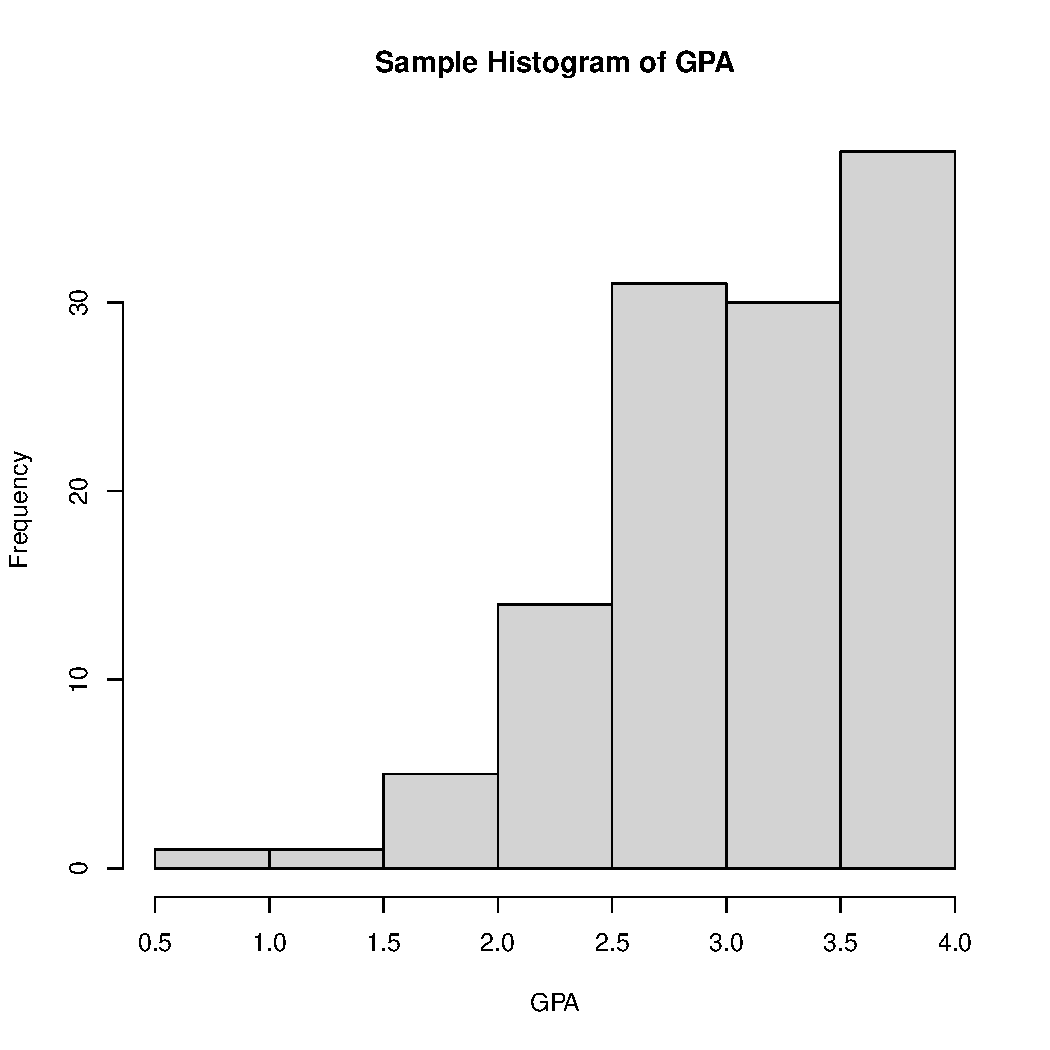
\includegraphics[width=0.6\textwidth]{figure/unnamed-chunk-2-1} 

\end{knitrout}

If you get the same results as the above, then your installation should be correctly setup and you will be good to go!

\section{R Basics}

Here is quick review of some basic skills you should be familiar with in R. If you feel comfortable doing all of the things below, then you should be just fine in this class.

\subsection{Running commands and scripts}

In RStudio, there are two places where you see code. You have a console, and you should also have a script window. By default, just the console window will be open. In there, you can type R commands and there will be ran in an interactive manner.

\begin{figure}[H]
  \centering
  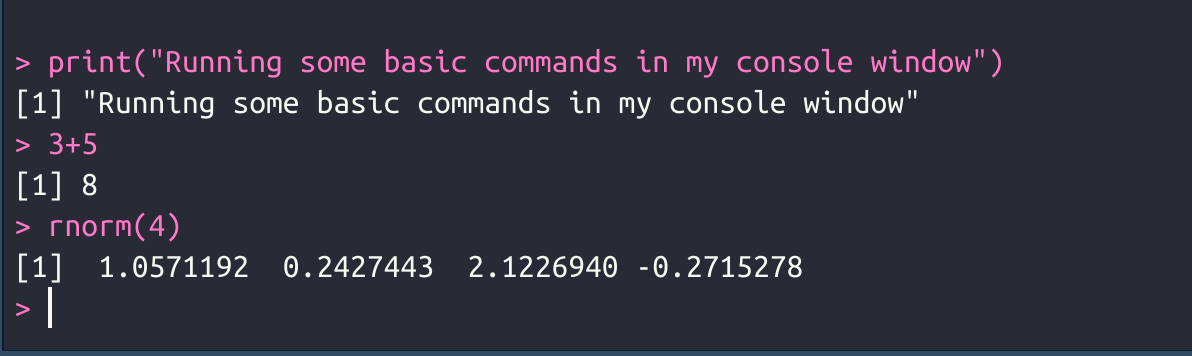
\includegraphics[width = 0.50\textwidth]{../figures/module1/rconsole1.png}
\end{figure}

You can also open R code inside a script window. If desired, you can run the entire R script. More often, you will be running bits and pieces of an R script at a time. Putting your code in a script has an advantage in that it's very easy to jump around your code and test little bits at a time without needing to type out your code every time.

If you go to File $\rightarrow$ Open File, you can open an R file inside RStudio. To run one chunk of code, select it with your mouse and then click either ``Run'' at the top right part of the script window, or Ctrl+Enter (my favorite method and much quicker than clicking run!)

\begin{figure}[H]
  \centering
  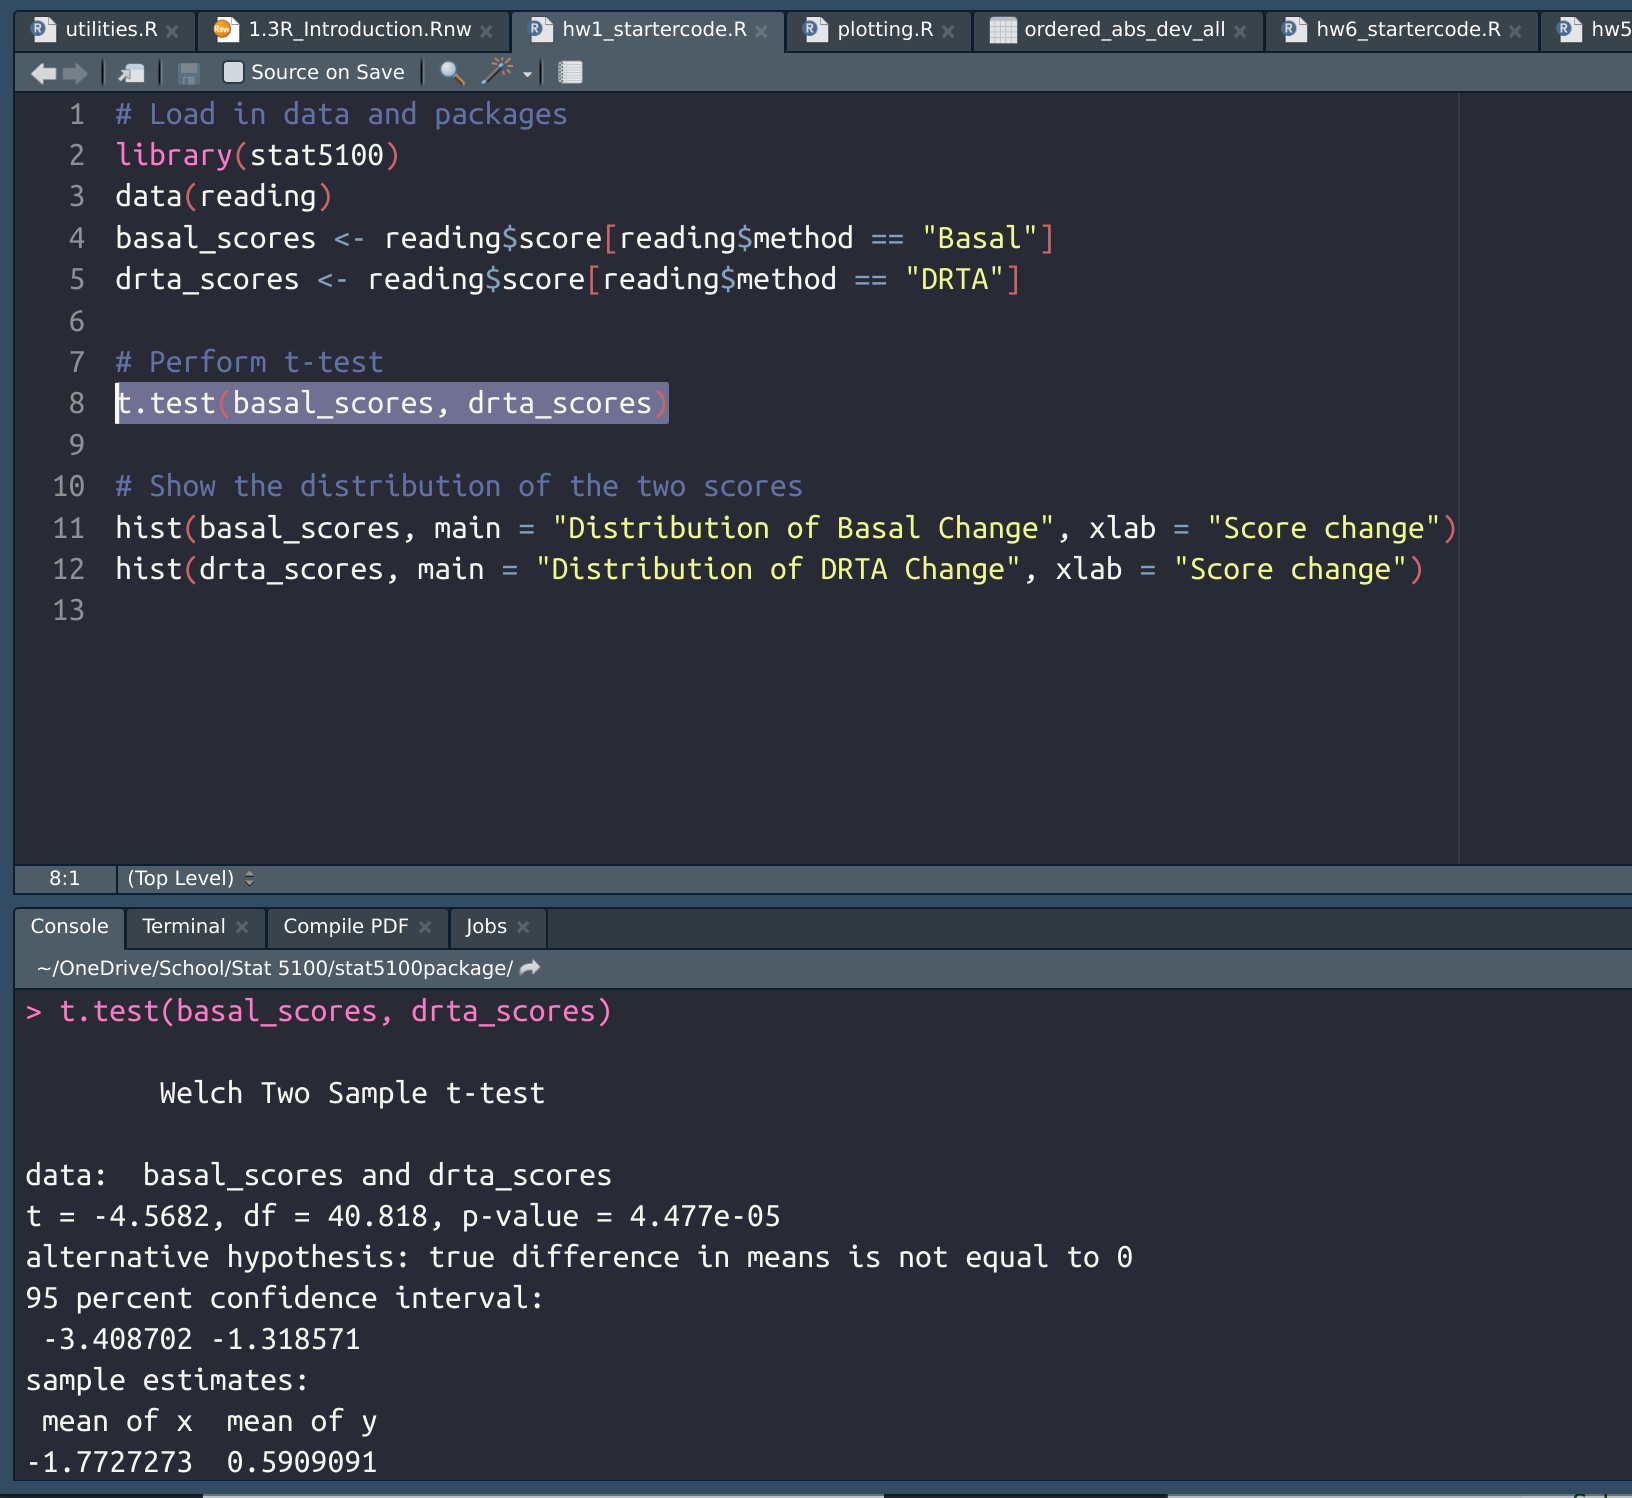
\includegraphics[width = 0.70\textwidth]{../figures/module1/rscriptrun1.png}
\end{figure}

\subsection{Getting help on functions}

Not even the best R programmers memorize how to use every single function. Very often, you will know that a function exists but you forget the exact parameters to enter and how to use the function. Fortunately, R has integrated a very easy help page lookup feature. To use this lookup feature, prepend the command you want to learn about with a question mark ``?'' and enter it into the console. For example, to get help on the stat5100::residual\_plot() function, type ``?stat5100residual\_plot'' into the console.

\begin{figure}[H]
  \centering
  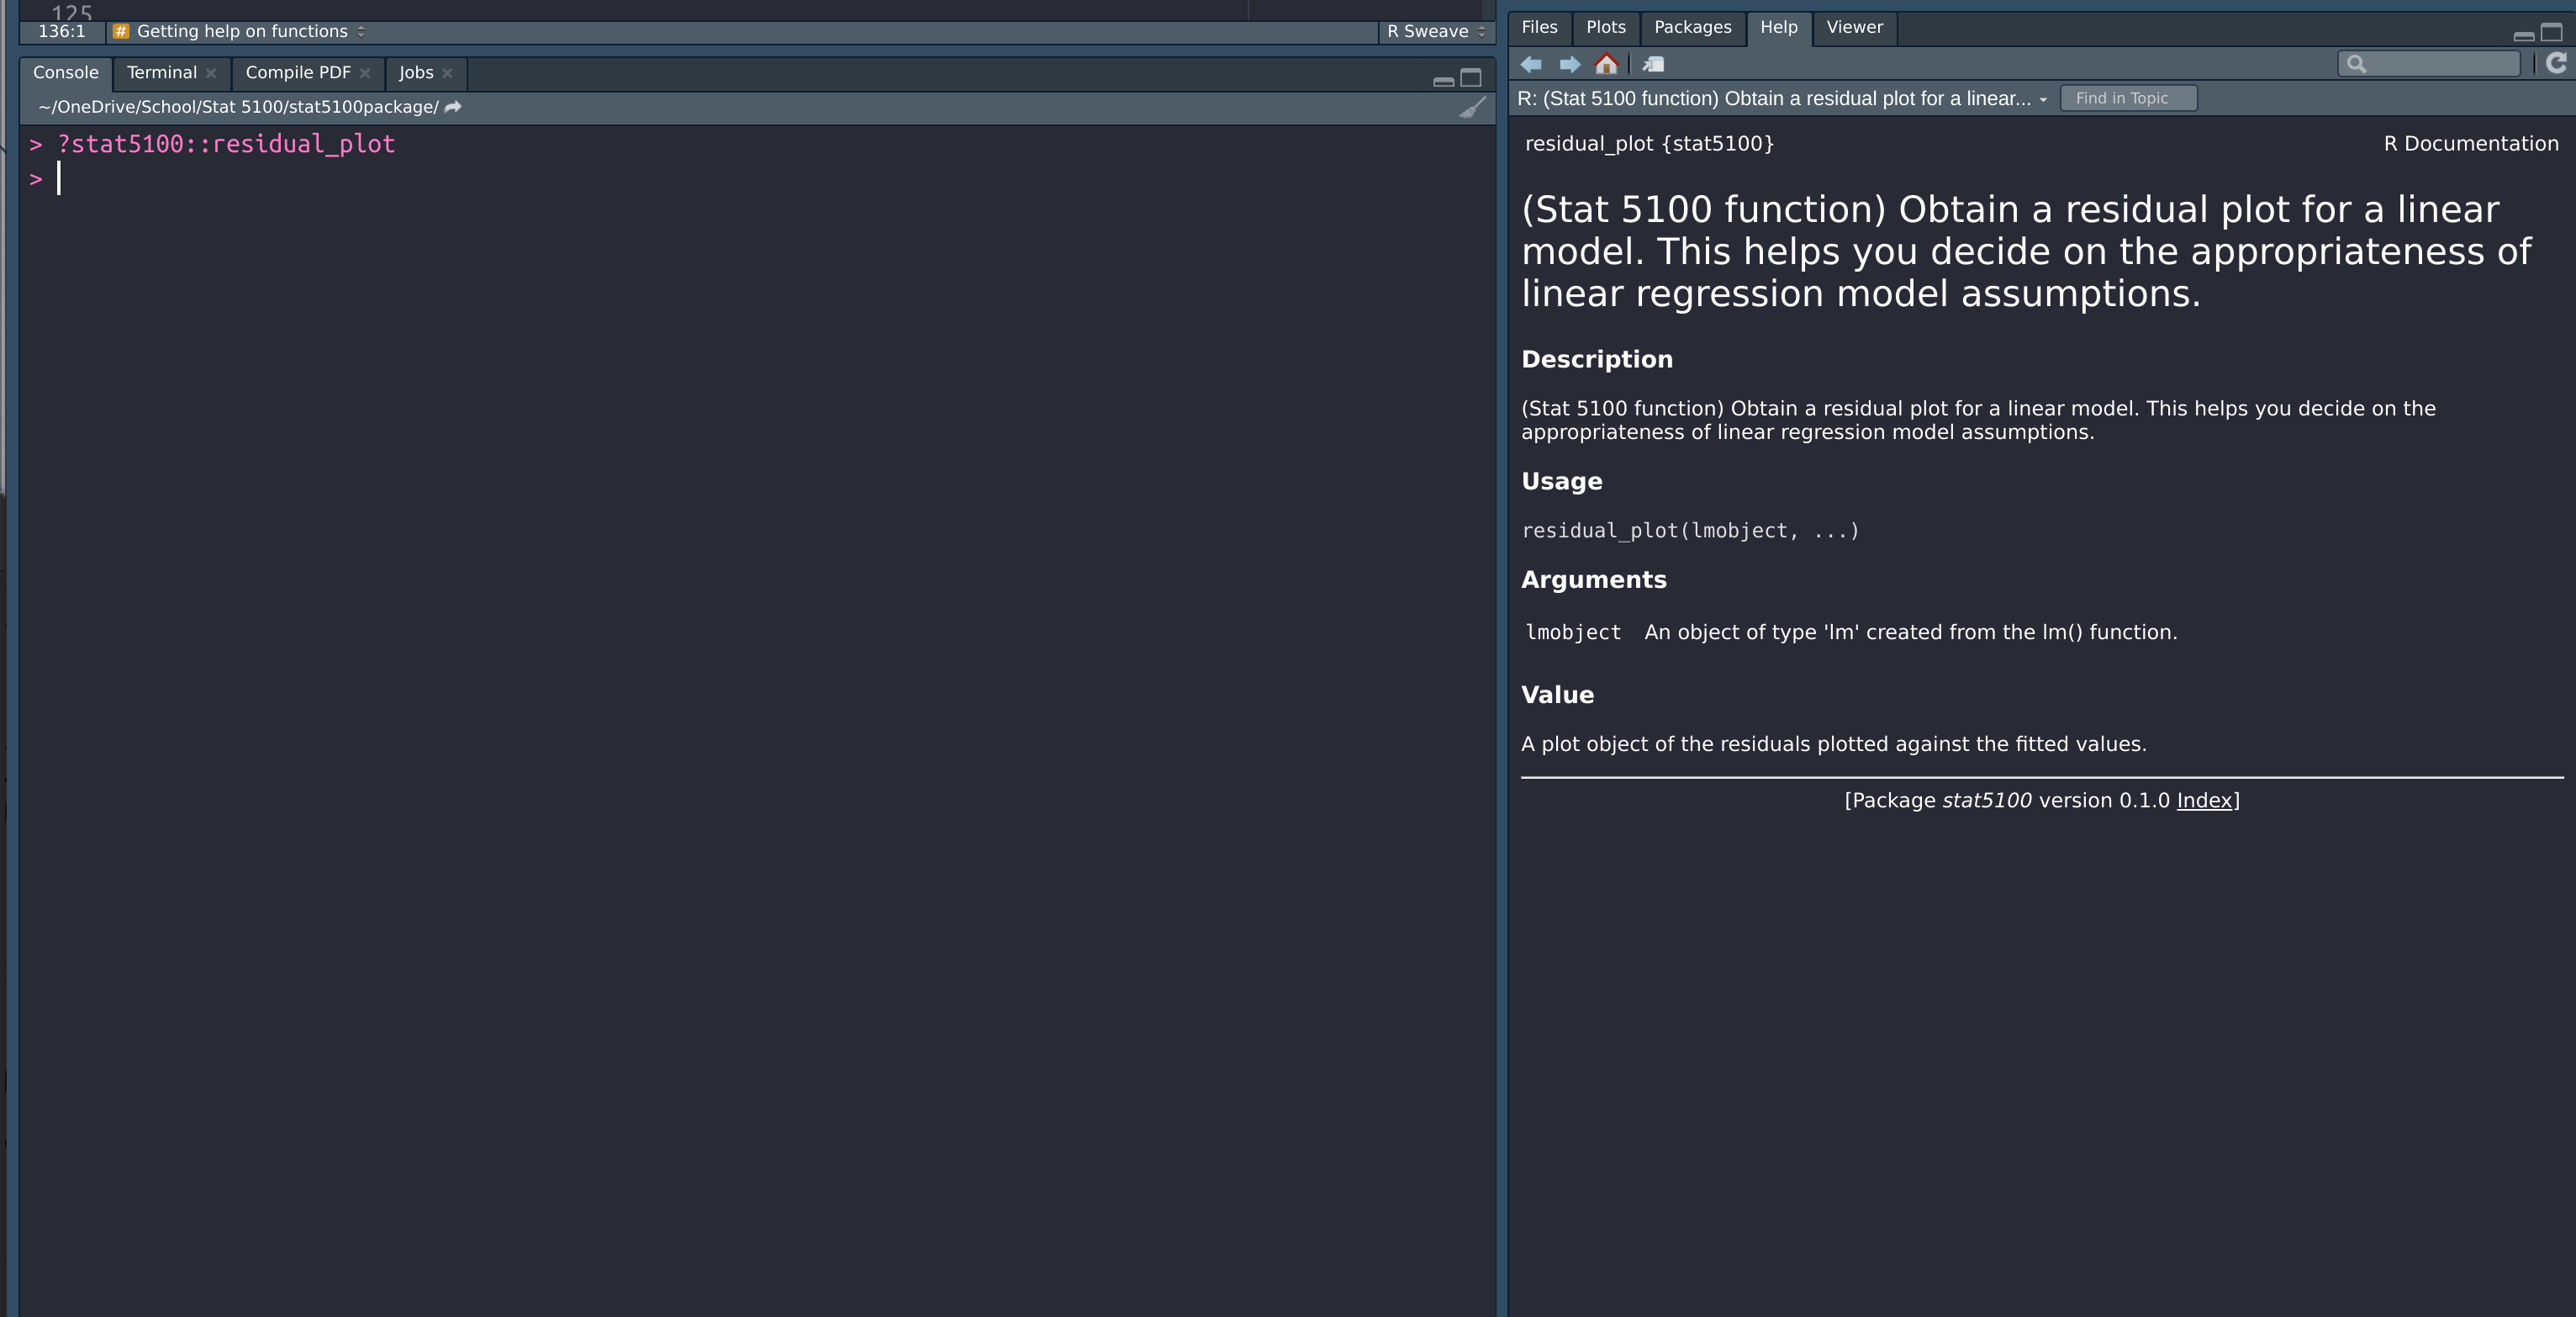
\includegraphics[width = 0.70\textwidth]{../figures/module1/rgettinghelp.png}
\end{figure}

Every single function that you will ever use in this class will come with a help page that can be accessed this way.

\subsection{Reading in data}
\subsubsection{Reading in Stat 5100 datasets}

Nearly all of the datasets that we use in this class (with a few exceptions) are made available right away in the stat5100package. To load them into memory, simply use the data() function with the name of the dataset in the parenthesis.

\begin{knitrout}
\definecolor{shadecolor}{rgb}{0.969, 0.969, 0.969}\color{fgcolor}\begin{kframe}
\begin{alltt}
\hlkwd{data}\hlstd{(surgical)}
\end{alltt}
\end{kframe}
\end{knitrout}

Note that for this to work, you \textit{must} have the Stat 5100 package loaded already:

\begin{knitrout}
\definecolor{shadecolor}{rgb}{0.969, 0.969, 0.969}\color{fgcolor}\begin{kframe}
\begin{alltt}
\hlkwd{library}\hlstd{(stat5100)}
\end{alltt}
\end{kframe}
\end{knitrout}

\subsubsection{Reading in data by CSV}

To read in a CSV file, it is a little bit more tricky but still very easy. To load a CSV file, we use the read.csv() function in R with the location of the file as a string inside the paranthesis. Note that this function requires we assign the CSV data to an object name.

\begin{knitrout}
\definecolor{shadecolor}{rgb}{0.969, 0.969, 0.969}\color{fgcolor}\begin{kframe}
\begin{alltt}
\hlstd{my_data_name} \hlkwb{<-} \hlkwd{read.csv}\hlstd{(}\hlstr{"../../../../data_csv/grocery.csv"}\hlstd{)}
\end{alltt}
\end{kframe}
\end{knitrout}

Note that the file location is specified relevant to your current working directory. To access a file that is ``up'' a directory, use .. to indicate this (you see this in the above command!)

To find out where your current working directory is, run the following:

\begin{knitrout}
\definecolor{shadecolor}{rgb}{0.969, 0.969, 0.969}\color{fgcolor}\begin{kframe}
\begin{alltt}
\hlkwd{getwd}\hlstd{()}
\end{alltt}
\begin{verbatim}
## [1] "/home/ethan/OneDrive/School/Stat 5100/teaching/Stat5100/notes/Module 1"
\end{verbatim}
\end{kframe}
\end{knitrout}

To set your working directory, you can use the setwd() function, but it is easier to go to Session $\rightarrow$ Set Working Directory $\rightarrow$ Choose Directory inside of RStudio.

\subsubsection{Creating data by hand}

Sometimes, we might need to create a dataframe by hand. Here is an example where we create a very dataframe and display its contents in the console:

\begin{knitrout}
\definecolor{shadecolor}{rgb}{0.969, 0.969, 0.969}\color{fgcolor}\begin{kframe}
\begin{alltt}
\hlstd{my_amazing_dataframe} \hlkwb{<-} \hlkwd{data.frame}\hlstd{(}\hlkwc{column_name1} \hlstd{=} \hlkwd{c}\hlstd{(}\hlstr{"Yellow"}\hlstd{,} \hlstr{"Blue"}\hlstd{,} \hlstr{"Red"}\hlstd{),}
                                   \hlkwc{some_numbers} \hlstd{=} \hlkwd{c}\hlstd{(}\hlnum{5}\hlstd{,} \hlnum{7}\hlstd{,} \hlnum{89}\hlstd{),}
                                   \hlkwc{more_numbers} \hlstd{=} \hlkwd{c}\hlstd{(}\hlnum{4}\hlstd{,} \hlnum{8}\hlstd{,} \hlnum{1}\hlstd{),}
                                   \hlkwc{some_logicals} \hlstd{=} \hlkwd{c}\hlstd{(}\hlnum{TRUE}\hlstd{,} \hlnum{TRUE}\hlstd{,} \hlnum{FALSE}\hlstd{))}

\hlstd{my_amazing_dataframe}
\end{alltt}
\begin{verbatim}
##   column_name1 some_numbers more_numbers some_logicals
## 1       Yellow            5            4          TRUE
## 2         Blue            7            8          TRUE
## 3          Red           89            1         FALSE
\end{verbatim}
\end{kframe}
\end{knitrout}


\subsection{Altering datasets}

There are a variety of ways we might want to alter a dataset:

\begin{knitrout}
\definecolor{shadecolor}{rgb}{0.969, 0.969, 0.969}\color{fgcolor}\begin{kframe}
\begin{alltt}
\hlcom{# Create a new column}
\hlstd{my_amazing_dataframe} \hlkwb{<-} \hlkwd{cbind}\hlstd{(my_amazing_dataframe,}
                              \hlkwc{muchos_numeros} \hlstd{= my_amazing_dataframe}\hlopt{$}\hlstd{some_numbers} \hlopt{*}
                                               \hlstd{my_amazing_dataframe}\hlopt{$}\hlstd{more_numbers,}
                              \hlkwc{numbers_exponent} \hlstd{= my_amazing_dataframe}\hlopt{$}\hlstd{some_numbers}\hlopt{^}\hlnum{5.5}\hlstd{)}

\hlstd{my_amazing_dataframe}
\end{alltt}
\begin{verbatim}
##   column_name1 some_numbers more_numbers some_logicals muchos_numeros
## 1       Yellow            5            4          TRUE             20
## 2         Blue            7            8          TRUE             56
## 3          Red           89            1         FALSE             89
##   numbers_exponent
## 1     6.987712e+03
## 2     4.446714e+04
## 3     5.267991e+10
\end{verbatim}
\begin{alltt}
\hlcom{# Set all instances of the number 1 inside the "more_numbers" column to be the}
\hlcom{# number e instead.}
\hlstd{my_amazing_dataframe}\hlopt{$}\hlstd{more_numbers[my_amazing_dataframe}\hlopt{$}\hlstd{more_numbers} \hlopt{==} \hlnum{1}\hlstd{]} \hlkwb{<-} \hlkwd{exp}\hlstd{(}\hlnum{1}\hlstd{)}

\hlstd{my_amazing_dataframe}
\end{alltt}
\begin{verbatim}
##   column_name1 some_numbers more_numbers some_logicals muchos_numeros
## 1       Yellow            5     4.000000          TRUE             20
## 2         Blue            7     8.000000          TRUE             56
## 3          Red           89     2.718282         FALSE             89
##   numbers_exponent
## 1     6.987712e+03
## 2     4.446714e+04
## 3     5.267991e+10
\end{verbatim}
\end{kframe}
\end{knitrout}


\subsection{Filtering datasets}

To conditionally access parts of a dataframe, you can run any of the following:
\begin{knitrout}
\definecolor{shadecolor}{rgb}{0.969, 0.969, 0.969}\color{fgcolor}\begin{kframe}
\begin{alltt}
\hlcom{# print all rows where "some_numbers" was 5}
\hlstd{my_amazing_dataframe[my_amazing_dataframe}\hlopt{$}\hlstd{some_numbers} \hlopt{==} \hlnum{5}\hlstd{, ]}
\end{alltt}
\begin{verbatim}
##   column_name1 some_numbers more_numbers some_logicals muchos_numeros
## 1       Yellow            5            4          TRUE             20
##   numbers_exponent
## 1         6987.712
\end{verbatim}
\begin{alltt}
\hlcom{# Print columns 1 and 3}
\hlstd{my_amazing_dataframe[,} \hlkwd{c}\hlstd{(}\hlnum{1}\hlstd{,}\hlnum{3}\hlstd{)]}
\end{alltt}
\begin{verbatim}
##   column_name1 more_numbers
## 1       Yellow     4.000000
## 2         Blue     8.000000
## 3          Red     2.718282
\end{verbatim}
\begin{alltt}
\hlcom{# Print all elements of some_numbers where some_numbers is either 5 or 7.}
\hlstd{my_amazing_dataframe}\hlopt{$}\hlstd{some_numbers[(my_amazing_dataframe}\hlopt{$}\hlstd{some_numbers} \hlopt{==} \hlnum{5} \hlopt{|}
                                    \hlstd{my_amazing_dataframe}\hlopt{$}\hlstd{some_numbers} \hlopt{==} \hlnum{7}\hlstd{)]}
\end{alltt}
\begin{verbatim}
## [1] 5 7
\end{verbatim}
\end{kframe}
\end{knitrout}


\section{Miscellaneous Notes and FAQ}

Here are some notes you should be aware of:

\begin{itemize}

  \item To create a comment in your code (lines in a script that are notes and not actual code), place a # right before what you want to say. You probably have seen this in some of the code examples above.

\end{itemize}

\subsubsection*{Other random questions:}

Q: Where is the best place to go for R help?

A: To be completely honest, the best place to ask questions about R is on Google. Most likely, any question you have has been asked by somebody else. Finding help for your code online is an incredibly important skill: anyone who programs in any capacity should become familiar with this skill eventually.

However, if you aren't finding what you need online or you want some human help, either the TA or the professor is very happy to answer your questions via email or office hours.

\bigskip

Q: Can I view all the R code that is in the Stat 5100 package?

A: Yes! If you are a more complex R user and you wish to see what is happening behind the scenes in some of these functions, then you are welcome to look in the source code of the R package to see what code lies behind these functions. For example, the ``visual\_assumptions()'' function in the code snippet above does not exist natively in R, it is a function that comes from the Stat 5100 R package.

To see the code on Github, navigate to \href{http://www.github.com/ethanancell/stat5100package}{http://www.github.com/ethanancell/stat5100package}. You are welcome to clone this repository or peek around the source code. All the R code is contained in the ``R'' folder, and is in either ``utilities.R'' or ``plotting.R.'' The plotting file should be very self-explanatory: it is where all the plotting functions we'll use in this class live. In utilities.R, we have more numerical methods for different complex calculations we will need for various things we do in this class.

Feel free to clone the repository and peek around. If you have any questions about the package for the course, feel free to direct them to me at ethanancell@aggiemail.usu.edu.
\end{document}
